% !TEX root = HW6.tex
% !TEX root = HW6.tex

\newcommand{\backpropStudSolA}{
%%%%%%%%%%%%%%%%%%%%%%%%%%%%%%%%%%%%
%%
%%.   YOUR SOLUTION FOR PROBLEM A BELOW THIS COMMENT
%%
%%%%%%%%%%%%%%%%%%%%%%%%%%%%%%%%%%%%
\begin{align*}
g\prime(x) &= \frac{d}{dx}\sigma (x)\\
&= \frac{d}{dx} (1 + e^{-x})^{-1}\\
&= -1 (1 + e^{-x})^{-2}e^{-x}(-1)\\
&= \frac{e^{-x}}{(1 + e^{-x})^{-2}}\\
&= \frac{1}{1 + e^{-x}} \frac{e^{-x}}{1 + e^{-x}}\\
&= \frac{1}{1 + e^{-x}} \frac{1+ e^{-x} - 1}{1 + e^{-x}}\\
&= \frac{1}{1 + e^{-x}} \left( 1 - \frac{1}{1 + e^{-x}} \right)\\
& = \sigma(x) \left(1 - \sigma(x) \right)\\
&= \sigma(x) - \sigma(x)^2
\end{align*}
}

\newcommand{\backpropStudSolB}{
%%%%%%%%%%%%%%%%%%%%%%%%%%%%%%%%%%%%
%%
%%.   YOUR SOLUTION FOR PROBLEM A BELOW THIS COMMENT
%%
%%%%%%%%%%%%%%%%%%%%%%%%%%%%%%%%%%%%
\begin{align*}
\delta_k &= \frac{\partial E}{\partial h_k}\\
&= \frac{\partial}{\partial h_k}
	\frac{1}{2}
	\sum_k \left( c_k - t_k \right)^2\\
&= \frac{\partial}{\partial h_k}
	\frac{1}{2} \left( c_k - t_k \right)^2\\
&= \left( c_k - t_k \right) \frac{\partial}{\partial h_k} c_k\\
&= \left( c_k - t_k \right) \frac{\partial}{\partial h_k} g \left( h_k \right)\\
&=  \left( c_k - t_k \right) g\prime(h_k)
\end{align*}
}

\newcommand{\backpropStudSolC}{
%%%%%%%%%%%%%%%%%%%%%%%%%%%%%%%%%%%%
%%
%%.   YOUR SOLUTION FOR PROBLEM A BELOW THIS COMMENT
%%
%%%%%%%%%%%%%%%%%%%%%%%%%%%%%%%%%%%%
\begin{align*}
\frac{\partial E}{\partial w_{jk}} &= \frac{\partial E}{\partial h_k} \frac{\partial h_k}{\partial w_{jk}}\\
&= \delta_k \frac{\partial h_k}{\partial w_{jk}}\\
&= \delta_k \frac{\partial}{\partial w_{jk}} \sum_j b_j w_{jk} + f_k\\
&= \delta_k \frac{\partial}{\partial w_{jk}} b_j w_{jk}\\
&= \delta_k b_j
\end{align*}
}

\newcommand{\backpropStudSolD}{
%%%%%%%%%%%%%%%%%%%%%%%%%%%%%%%%%%%%
%%
%%.   YOUR SOLUTION FOR PROBLEM A BELOW THIS COMMENT
%%
%%%%%%%%%%%%%%%%%%%%%%%%%%%%%%%%%%%%
\begin{align*}
\frac{\partial E}{\partial f_k} &= \frac{\partial E}{\partial h_k} \frac{\partial h_k}{\partial f_k}\\
&= \delta_k \frac{\partial}{\partial f_k} \sum_j b_j w_{jk} + f_k\\
&= \delta_k 
\end{align*}
}

\newcommand{\backpropStudSolE}{
%%%%%%%%%%%%%%%%%%%%%%%%%%%%%%%%%%%%
%%
%%.   YOUR SOLUTION FOR PROBLEM A BELOW THIS COMMENT
%%
%%%%%%%%%%%%%%%%%%%%%%%%%%%%%%%%%%%%
Note that $$b_j = g(z_j)$$.
\begin{align*}
\frac{\partial E}{\partial z_j} &= 
	\sum_k 
		\frac{\partial E}{\partial h_k}
		\sum_j
			\frac{\partial h_k}{\partial b_j}
			\frac{\partial b_j}{\partial z_j}\\
&= \sum_k
		\delta_k 
		\sum_j
			\frac{\partial h_k}{\partial b_j}
			\frac{\partial b_j}{\partial z_j}\\
&= \sum_k
		\delta_k
		\frac{\partial h_k}{\partial b_j}
		\frac{\partial b_j}{\partial z_j}\\
&= \sum_k
		\delta_k
		w_{jk}
		g\prime(z_j)\\
&= g\prime(z_j) \sum_k
		\delta_k
		w_{jk}
\end{align*}
}


\newcommand{\backpropStudSolF}{
%%%%%%%%%%%%%%%%%%%%%%%%%%%%%%%%%%%%
%%
%%.   YOUR SOLUTION FOR PROBLEM A BELOW THIS COMMENT
%%
%%%%%%%%%%%%%%%%%%%%%%%%%%%%%%%%%%%%
Note that 
\[ \frac{\partial z_j}{\partial u_{ij}} =  \frac{\partial}{\partial u_{ij}} \left( e_j + \sum_i a_i u_{ij} \right) = a_i \]
Now
\begin{align*}
\frac{\partial E}{\partial u_{ij}} &= \frac{\partial E}{\partial z_j} \frac{\partial z_j}{\partial u_{ij}}\\
&= \psi_j a_i
\end{align*}
}



\newcommand{\backpropStudSolH}{
%%%%%%%%%%%%%%%%%%%%%%%%%%%%%%%%%%%%
%%
%%.   YOUR SOLUTION FOR PROBLEM A BELOW THIS COMMENT
%%
%%%%%%%%%%%%%%%%%%%%%%%%%%%%%%%%%%%%
Note that 
\[ \frac{\partial z_j}{\partial e_j} =  \frac{\partial}{\partial e_j} \left( e_j + \sum_i a_i u_{ij} \right) = 1 \]
\begin{align*}
\frac{\partial E}{\partial e_j} &= \frac{\partial E}{\partial z_j} \frac{\partial z_j}{\partial e_j}\\
&= \psi_j 
\end{align*}
}
 %The students have to fill this file to print the solution

% Problem Explanation:
% - first argument is the number of points
% - second argument is the title and the text
\examproblem{8}{Backpropagation
}


Consider the deep net in the figure below consisting of an input layer, an output layer, and a hidden layer. The feed-forward computations performed by the deep net are as follows: every input $a_{i}$ is multiplied by a set of fully-connected weights $u_{ij}$ connecting the input layer to the hidden layer. The resulting weighted signals are then summed and combined with a bias $e_{j}$. This results in the activation signal $z_{j}=e_{j}+\sum_{i}a_{i}u_{ij}$. The hidden layer applies activation function $g$ on $z_{j}$ resulting in the signal $b_{j}$.  In a similar fashion, the hidden layer activation signals $b_{j}$ are multiplied by the weights connecting the hidden layer to the output layer $w_{jk}$, a bias $f_{k}$ is added and the resulting signal $h_{k}$ is transformed by the output activation function $g$ to form the network output $c_{k}$. The loss between the desired target $t_{k}$ and the output $c_{k}$ is given by the MSE: $E= \frac{1}{2} \sum_{k} (c_{k}-t_{k})^{2}$, where $t_{k}$ denotes the ground truth signal corresponding to $c_{k}$. Training a neural network involves determining the set of parameters $\theta=\{\emph{U},\emph{W},\emph{e},\emph{f}\}$ that minimize $E$. This problem can be solved using gradient descent, which requires determining $\frac{\partial E}{\partial \theta}$ for all $\theta$ in the model.


\begin{center}
 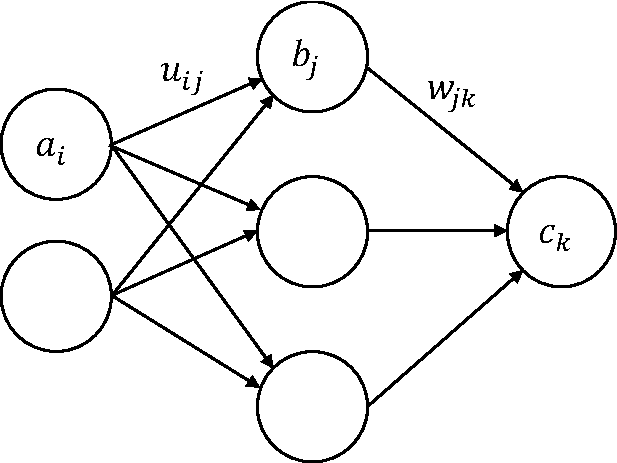
\includegraphics[width=7cm]{fig/DeepNet.pdf}
 \end{center}

%%%%%%%%%%%%%%%%%%%%%%%%%%%%%%%%%%%%%%
%%%%%  BEGINNING OF SUBPROBLEMS LIST
\begin{enumerate}

% Subproblem description
\examproblempart{ For $g(x)=\sigma(x)=\frac{1}{1+e^{-x}}$, compute the derivative $g'(x)$ of $g(x)$ as a function of $\sigma(x)$.}
\bookletskip{0}   %in inches

% Solution box 
 \framebox[14.7cm][l]{
 \begin{minipage}[b]{14.7cm}
\inbooklet{Your answer: \backpropStudSolA}
  
 \solution{\backpropSolA}

 \end{minipage}
 }

% Subproblem description
\examproblempart{ We denote by $\delta_{k}=\frac{\partial E}{\partial h_{k}}$ the error signal of neuron $k$ in the second linear layer of the network. Compute $\delta_{k}$ as a function of $c_k$, $t_k$, $g'$ and $h_k$.\\ }
\bookletskip{0}   %in inches

% Solution box 
 \framebox[14.7cm][l]{
 \begin{minipage}[b]{14.7cm}
\inbooklet{Your answer: \backpropStudSolB}
  
 \solution{\backpropSolB}

 \end{minipage}
 }

% Subproblem description
\examproblempart{ Compute $\frac{\partial E}{\partial w_{jk}}$. Use $\delta_k$ and $b_j$.\\}
\bookletskip{0.0}   %in inches

% Solution box 
 \framebox[14.7cm][l]{
 \begin{minipage}[b]{14.7cm}
 \inbooklet{Your answer: \backpropStudSolC}
  
 \solution{\backpropSolC}
  \end{minipage}
  }

% Subproblem description
\examproblempart{Compute $\frac{\partial E}{\partial f_{k}}$. Use $\delta_{k}$.\\}
\bookletskip{0.0}   %in inches

% Solution box 
 \framebox[14.7cm][l]{
 \begin{minipage}[b]{14.7cm}
 \inbooklet{Your answer: \backpropStudSolD}
  
 \solution{\backpropSolD}
 \end{minipage}
 }

% Subproblem description
\examproblempart{We denote by $\psi_{j}=\frac{\partial E}{\partial z_{j} }$ the error signal of neuron $j$ in the first linear layer of the network. Compute $\psi_{j}$ as a function of $\delta_{k}$, $w_{jk}$, $g'$ and $z_{j}$.\\ }
\bookletskip{0}   %in inches

% Solution box 
 \framebox[14.7cm][l]{
 \begin{minipage}[b]{14.7cm}
 \inbooklet{Your answer: \backpropStudSolE}
  
 \solution{\backpropSolE}
 \end{minipage}
 }
 
 
 % Subproblem description
\examproblempart{Compute $\frac{\partial E}{\partial u_{ij}}$. Use $\psi_{j}$ and $a_i$.\\ }
\bookletskip{0}   %in inches

% Solution box 
 \framebox[14.7cm][l]{
 \begin{minipage}[b]{14.7cm}
 \inbooklet{Your answer: \backpropStudSolF}
  
 \solution{\backpropSolF}
 \end{minipage}
 }
 
 
  % Subproblem description
\examproblempart{Compute $\frac{\partial E}{\partial e_{j}}$. Use $\psi_{j}$.\\ }
\bookletskip{0}   %in inches

% Solution box 
 \framebox[14.7cm][l]{
 \begin{minipage}[b]{14.7cm}
 \inbooklet{Your answer: \backpropStudSolH}
  
 \solution{\backpropSolH}
 \end{minipage}
 }
 
 
 %%%%%%%%%%%% END OF SUBPROBLEMS LIST

\end{enumerate}